%# -*- coding: utf-8-unix -*-
%%==================================================
%% chapter02.tex for SJTU Master Thesis
%%==================================================

\chapter{SCache的实现}
\label{chap:impl}

本章将展现SCache系统的实现概况。
SCache是一个用Java和Scala语言开发的,开源的shuffle数据管理系统,并且提供了一个对于DAG任务预调度的附属调度器。
同时SCache还在设计时提供了跨框架的接口,来实现对于现有主流分布式DAG计算框架的shuffle优化。
在这次实现中,我们以Spark作为DAG计算框架的实例来阐述在SCache辅助下分布式DAG计算框架的新的计算流程。
我们首先在章节\ref{sec:overview}中介绍了系统设计的概要。
之后的章节分别介绍水塘采样算法,SCache在容错性上的取舍,以及计算框架在适配SCache时的工程上的开销和可行性分析。

\section{系统设计概要}
\label{sec:overview}

SCache在系统层面上主要包含三个部件:一个分布式的shuffle数据管理系统,一个DAG的附属调度器,和一个Spark系统内部的守护进程。
如图\ref{fig:arch}所示,SCache采用了类似于GFS\cite{gfs}经典的主从节点架构来实现对shuffle数据在集群中的管理。

\begin{figure}[!htp]
	\centering
	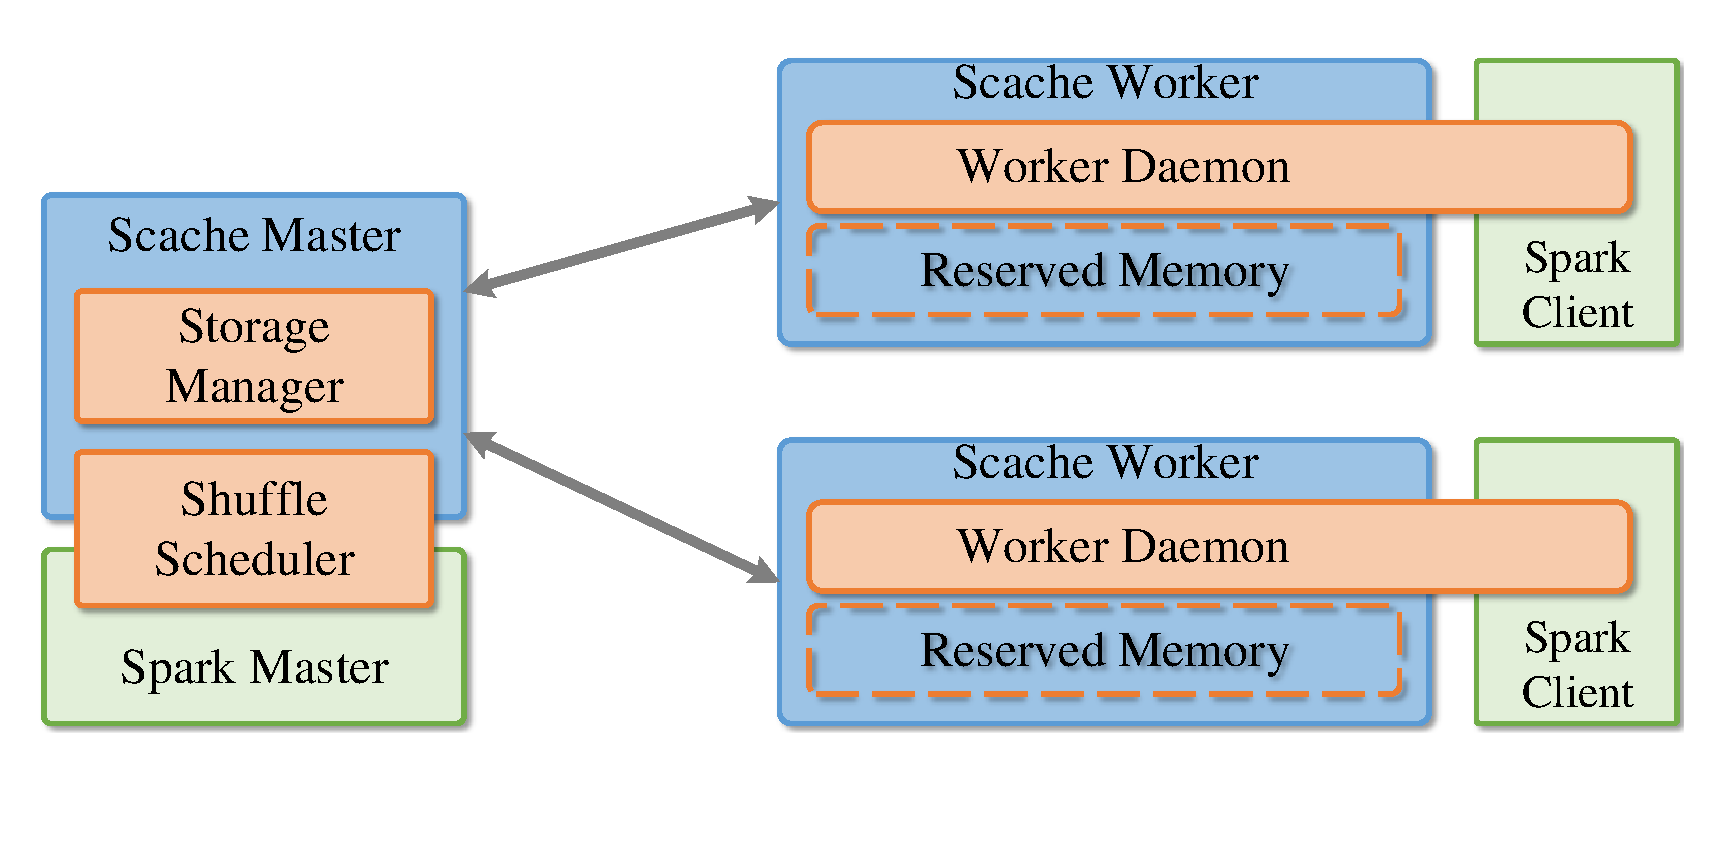
\includegraphics[width=0.8\textwidth]{../../PPoPP-2018/fig/arch.pdf}
	\bicaption[fig:arch]{SCache系统架构示意图}{SCache系统架构示意图}{Fig}{SCache Architecture}
\end{figure}

SCache的主节点负责管理整个分布式系统中的shuffle数据块预取与内存管理。
SCache的主节点中包含了DAG附属调度器,并且通过DAG附属调度器获取Spark上连接shuffle的reduce阶段任务预调度信息,任务的预调度执行顺序等。
此后SCache的主节点会将reduce阶段任务的预调度信息通知到各个从属工作节点。
当工作节点收到任务预调度信息之后,会立刻开始对远程已经完成的map任务进行shuffle数据的预取。
并且对于未完成的map任务,一旦工作节点通过内存拷贝的方式获取了相应的shuffle数据后就立即广播给集群中的各个节点,以便其开始shuffle的预取。
除此之外,SCache主节点还会根据任务的执行顺序信息给各个shuffle的数据单元标注上优先级并且发送给各个工作节点。

SCache的工作节点会在本地占用一部分内存空间用来存储shuffle的数据块。
为了减少内存管理的开销,SCache使用了Java虚拟机的堆外内存来对shuffle的数据块进行存储。
采用这种方式,既可以减少序列化反序列化带来的计算资源开销,同时又减轻了Java虚拟机垃圾回收算法(Garbage Collection)中的计算复杂度,有利于提升系统的整体性能。

与此同时,当本地的内存空间不够时,各个工作节点会根据从主节点收到的shuffle数据块优先级信息,结合本地的缓存信息(比如是否存在不完整的shuffle存储单元)来将一部分shuffle数据先保存到磁盘上。
本地的工作节点会在内存中至少缓存一个优先级最高的reduce任务需要的shuffle数据块。
当本地工作节点的shuffle缓存数据被任务消耗时,该部分内存空间就会被释放,而在磁盘中缓存的较高优先级的数据就会被立刻放入内存中。
通过结合主节点的优先级信息,本地shuffle的缓存状况以及Spark任务对shuffle数据的访问状况,工作节点的调度可以保证相对独立的完成内存管理并且保证:(1)shuffle数据可以在reduce任务开始执行前就被缓存在内存当中并且(2)shuffle数据的内存缓存不会破坏全部或没有以及应用优先级的限制。

SCache中的DAG附属调度器主要负责从Spark的Driver中获取DAG的信息,包括相邻map阶段和reduce阶段之间shuffle的数目,map任务的个数和reduce任务的个数以及当前map任务的shuffle输出的数据分别或者采样任务之后的数据分布。
DAG附属调度器会根据以上信息采用相应的线性回归算法或者采样算法来预测shuffle数据的分布,同时调用算法\ref{mhminheap}和算法\ref{hminheap}来作出一个启发式的reduce任务预调度。
在获得最终调度结果之后,附属调度器会将调度结果发送给SCache的主节点。
同时该调度结果也会在Spark任务调度器调度reduce阶段的任务之前将预调度的结果发送到任务调度器上。

守护进程以一个独立线程的形式存在于Spark的内存空间,通过远程过程调用(Remote Procedure Call,RPC)的方式与SCache进行通信。
守护进程同时还负向Spark系统内部的具体执行map任务和reduce任务的线程以及Spark任务调度器和Driver提供SCache相应的接口。

\begin{table}[!hpb]
    \centering
    \bicaption[tab:apis]{SCache编程接口列表}{SCache编程接口列表}{Table}{API list of SCache}
    \begin{tabular}{ | m{2.5cm} | m{8cm} | m{5cm} | }
        \hline
        接口 & 参数 & 作用 \\ [0.5ex]
        \hline
        \hline
        registerShuffles & jobId: Int, shuffleIds: Array[Int], maps: Array[Int], reduces: Array[Int], partitioner: Array[String] & 向SCache注册shuffle \\ \hline
        getBlock & blockId: String & 向SCache获取shuffle的数据块 \\ \hline
        putBlock & blockId: String, data: Array[Byte], len: Int & 向SCache发送shuffle数据块 \\ \hline
        getShuffleStatus & jobId: Int, shuffleId: Int & 向SCache获取reduce任务的预调度结果 \\ \hline
        sampling & jobId: Int, shuffleId: Int, distribution: Array[Array[Float]] & 向SCache发送采样分布 \\ 
        \hline
    \end{tabular}
\end{table}

\section{工作流程}

接下来我们将介绍在SCache的协同下Spark执行DAG的工作流程。
工作流程的第一阶段如图\ref{fig:regshuffle}所示,SCache需要首先从Spark中获取DAG的具体信息。

\begin{figure}[!htp]
	\centering
	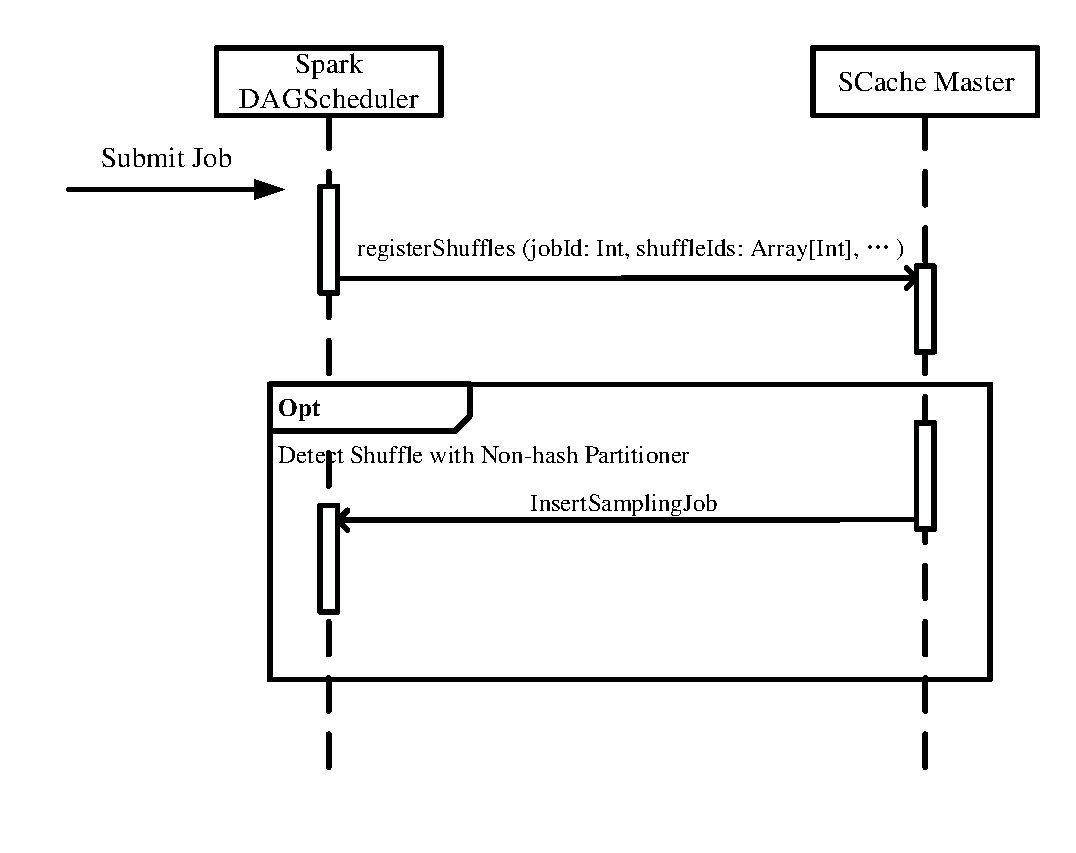
\includegraphics[width=0.8\textwidth]{shuffleregflow.pdf}
	\bicaption[fig:regshuffle]{注册shuffle时序图}{注册shuffle时序图}{Fig}{Sequence Diagram of Shuffle Registration}
\end{figure}

当一个Spark的工作启动时,首先会根据用户的代码生成一个关于RDD(Resilient Distributed Datasets)的系带关系(lineage)。
之后Spark的调度器会从最终的用户RDD递归向前寻找依赖的RDD。
在RDD之间的数据依赖中,如果存在部分依赖,也就是shuffle依赖,Spark会在此处插入一个shuffle过程,并且将之前的所有RDD合并成一个计算阶段(stage)。
递归寻找的过程会在当一个RDD的数据已经被计算或者已经到了存储系统的部分就会停止。
而这些计算阶段则最终组成了计算过程中的DAG逻辑。

对于DAG中相邻计算阶段之间的shuffle依赖,它们会被打包成一个RPC的调用提交到SCache的从属调度器上。如表\ref{tab:apis}中,一个shuffle依赖需要包含一个唯一的整数ID代表该Spark应用程序。
同时该RPC还需要包含这个shuffle依赖中每个shuffle的ID,以及它们对应的分区函数的类型,map阶段任务数和reduce阶段的任务数。
在收到注册shuffle的RPC之后,SCache的DAG附属调度器会首先检查分区函数的类型,如果不是哈希分区函数,就会通过在Spark的Driver上的守护进程在Spark执行该计算阶段前插入一段采样程序。
我们会在章节\ref{sec:sampling}和章节\ref{sec:impl}中详细阐述这个过程。

在之后的map计算阶段任务执行与shuffle数据收集过程中的时序图如图\ref{fig:putblock}所示。

\begin{figure}[!htp]
	\centering
	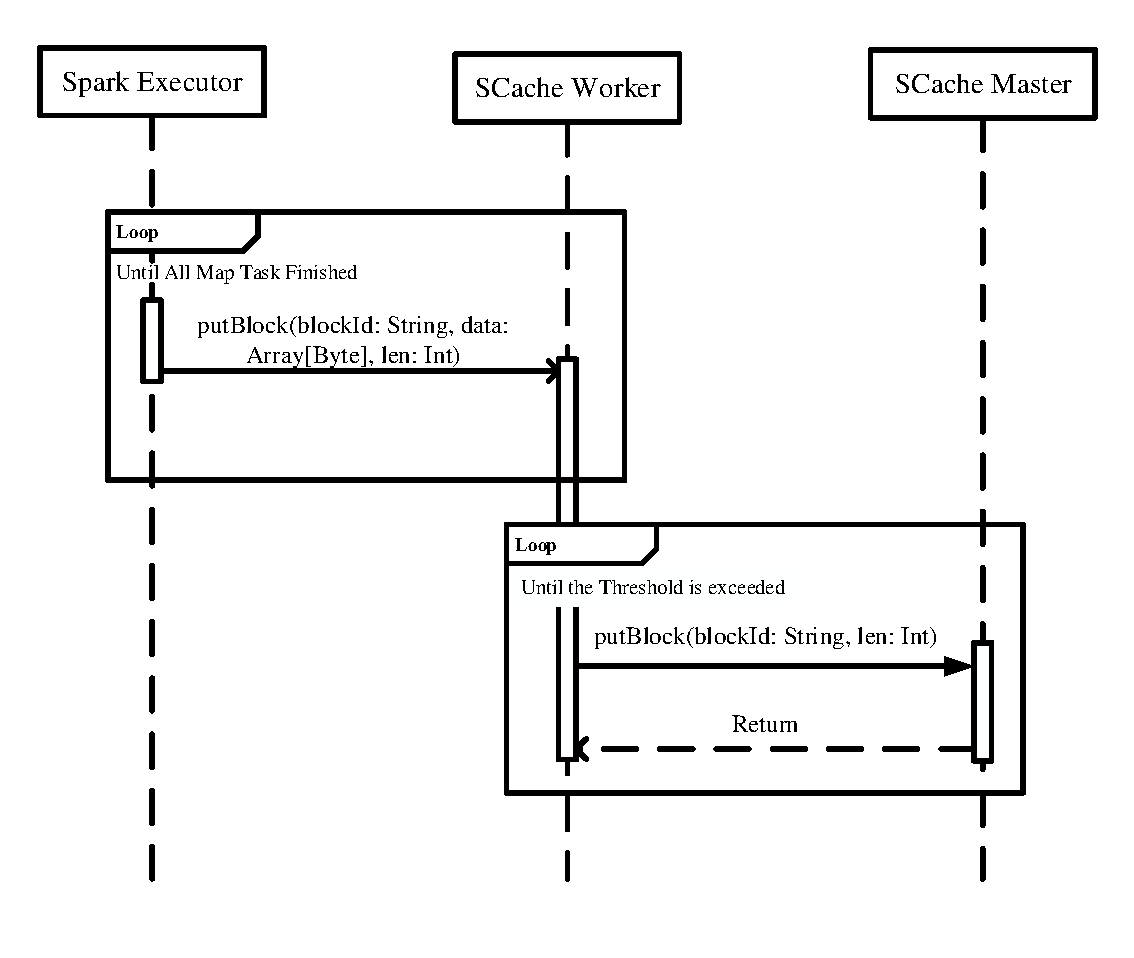
\includegraphics[width=0.8\textwidth]{putblock.pdf}
	\bicaption[fig:putblock]{Map阶段shuffle数据收集时序图}{Map阶段shuffle数据收集时序图}{Fig}{Sequence Diagram of Shuffle Data Collection in Map Stage}
\end{figure}

对于一个哈希分区函数的map任务,当计算结束之后分区函数会将计算产生的键值对通过相应的哈希函数划分成不同的数据块。
对于每一个数据块,SCache在Spark系统中的daemon程序都会根据其所在的工作ID对应的shuffle依赖ID,map任务ID,和reduce任务ID对每个数据块进行一个唯一的编号(即表格\ref{tab:apis}中的blockId)。
在此之后daemon程序会首先通过RPC的方式将这些shuffle数据块的元数据发送给SCache本地节点的工作进程。
与此同时,daemon进程也会通过Java对象的序列化的方式,将相应的数据序列化成字节码。
当接受到元数据之后,SCache的本地进程就会通过内存拷贝的形式,将序列化之后的字节码数据从Spark执行器的Java虚拟机的内存空间通过daemon程序拷贝到外部SCache的内存空间。
一旦内存拷贝结束,该map任务所占用的计算资源(slot)就会被立即释放。
通过SCache此处的内存拷贝优化,使得原先阻塞的磁盘I/O操作被避免,从而实现了map任务端更细粒度的硬件资源管理,提高了硬件资源的利用率和复用率。

在SCache的本地进程获取了该map任务输出的shuffle数据块之后,它会通过SCache系统内部的RPC接口通知SCache的主节点,并且在通知中附上了该map任务对于所有reduce任务产生的shuffle数据块大小(如图\ref{fig:shuffle}中的“map output”)。
每个数据块的大小可以通过内存拷贝时每个“blockId”对应的字节数组的长度来获得(即接口\ref{tab:apis}中putBlock的参数len: Int)。
当SCache的主节点收到了足够多的shuffle数据块信息之后(该threshold可以通过配置文件更改),会通过线性回归模型首先对reduce任务的输入数据分布进行预测。
之后DAG附属调度器会根据对shuffle的预测数据,调用算法\ref{mhminheap}和算法\ref{hminheap}来对redcue任务进行预调度。

\begin{figure}[!htp]
	\centering
	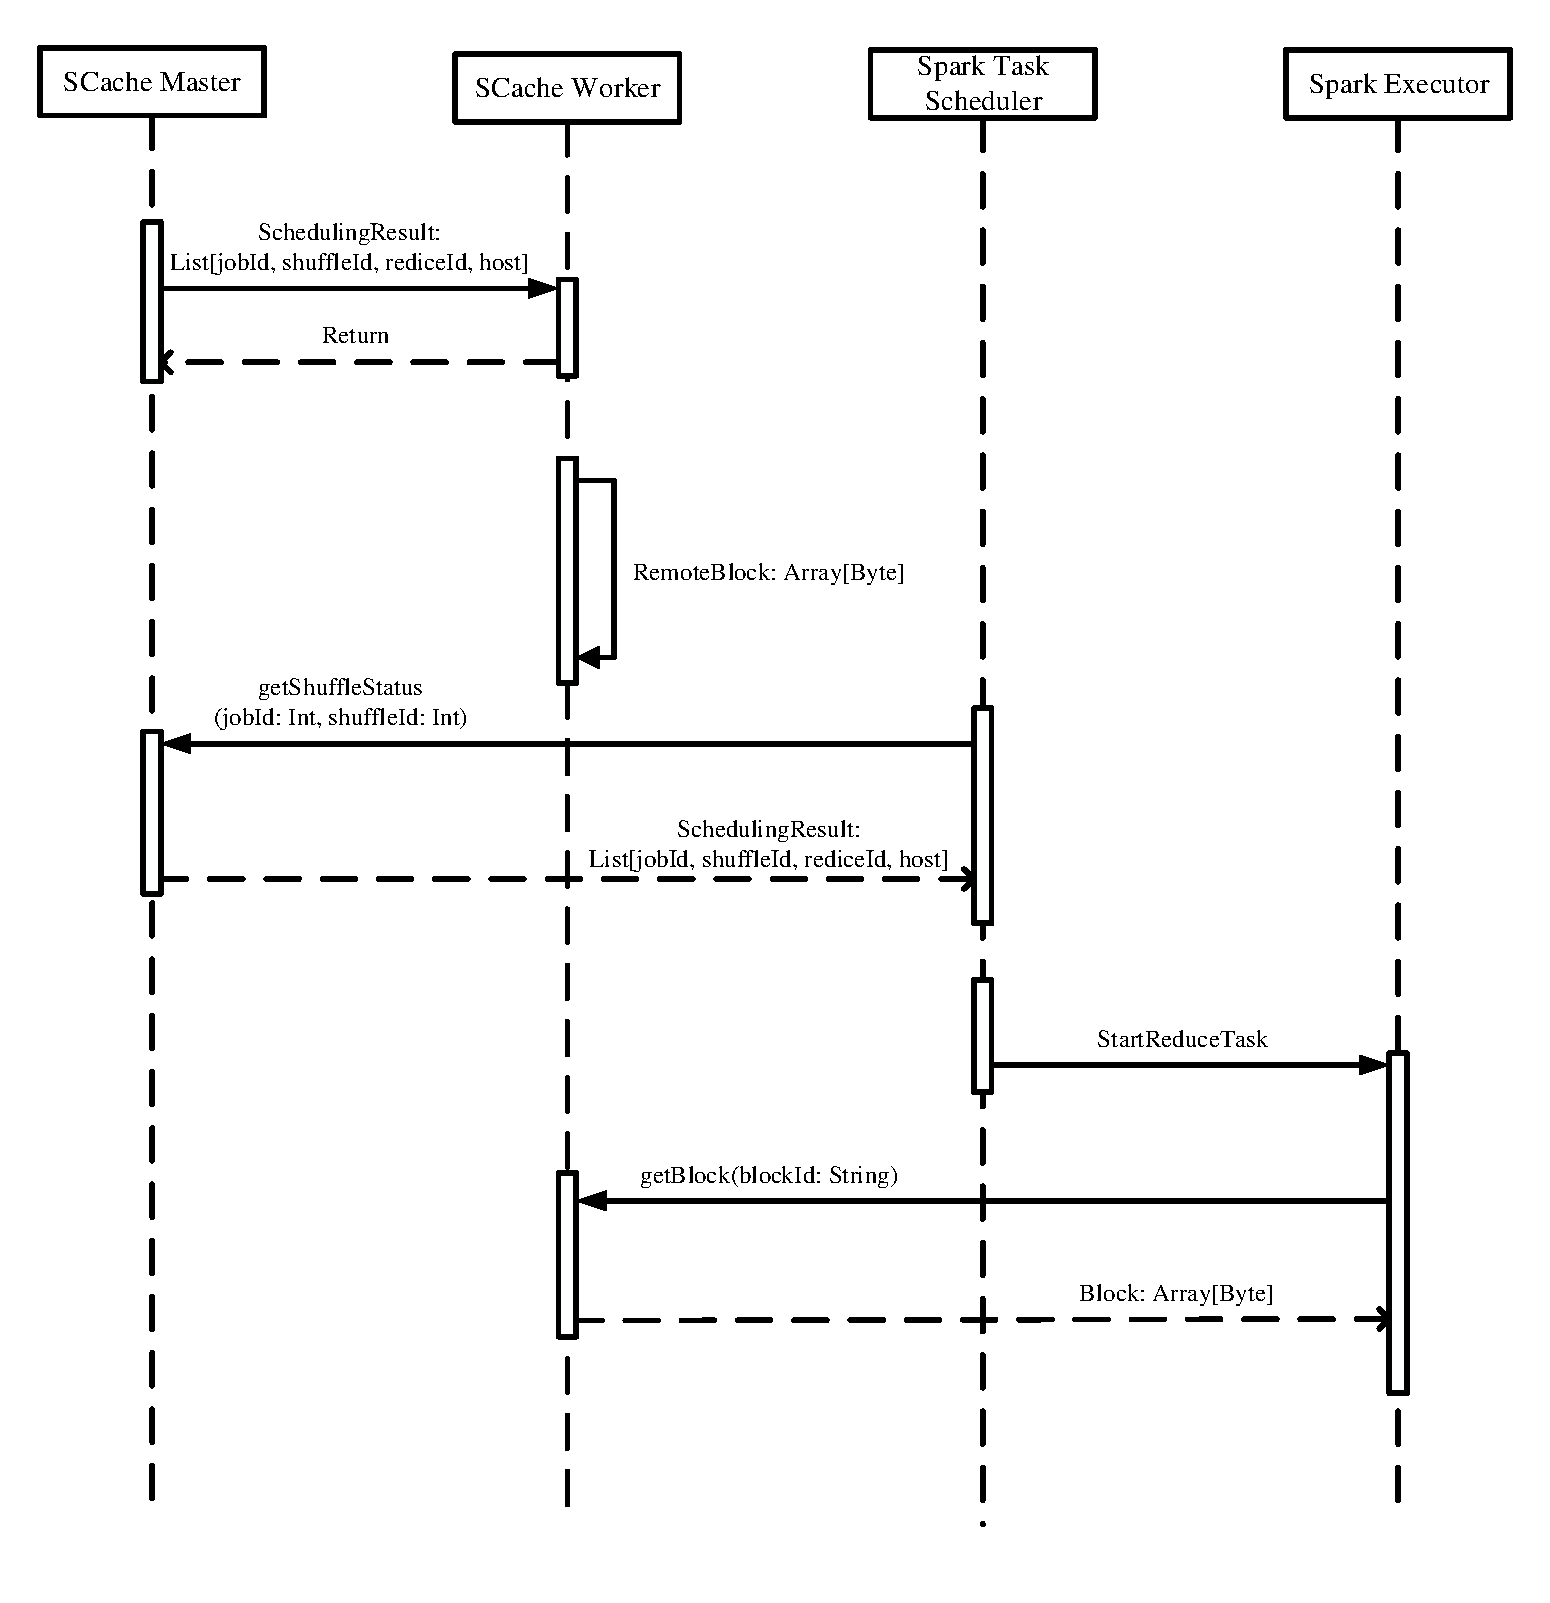
\includegraphics[width=0.8\textwidth]{preschedule.pdf}
	\bicaption[fig:preschedule]{预调度与预取工作时序图}{预调度与预取工作时序图}{Fig}{Sequence Diagram of Pre-scheduling and Pre-fetching}
\end{figure}

在SCache的中心节点完成预调度之后的流程具体如图\ref{fig:preschedule}所示。
当预调度算法运行结束之后,SCache的主节点会将reduce任务与计算节点的映射关系进行广播。
每个工作节点的SCache进程收到预调度的信息之后,会根据节点信息做出筛选,选出需要在本地执行的reduce任务。
此后本地节点会根据相应的工作ID,shuffle依赖ID,map任务ID,以及即将在本地执行的reduce任务ID组合而成的blockId,查询获取该数据块所在的节点位置,之后便开始从该远程节点预取数据。
当一个数据块被预取之后,其在节点的内存缓存就会被释放。

在reduce任务被调度的阶段,为了使Spark任务调度器遵循SCache的预调度结果,我们修改Spark的DAG调度器,通过表\ref{tab:apis}中getShuffleStatus的接口获取SCache预调度的任务 --- 节点映射关系。
在此基础上,我们将reduce任务中分配的节点修改成预调度的结果,从而使redcue任务在执行过程中获得shuffle数据预取与内存缓存的优化。

\section{水塘抽样}
\label{sec:sampling}

在上文的工作流程中,如果在注册shuffle时SCache检测到不是哈希分区函数,则SCache部署在Spark主节点上的守护进程会在使用非哈希分区函数的RDD中调用其$mapPartitionsWithIndex$\cite{sparksource}方法对每个分区的数据进行水塘采样。
如图\ref{fig:sample}所示,对于每个计算节点的本地采样程序,我们使用了经典的水塘采样算法\cite{reservoir},对每个数据分区中的输入数据进行随机采样计算并且统计经过分区函数分区后的输出shuffle数据分布。
在具体实现中,对于采样的样本数,我们将其设置为“$3 \times $数据块数目”,以此来平衡采样的精确度和采样的开销。
此处采样的样本数可以根据用户配置进行调整。
在对任务数据进行采样的同时,算法也会统计该数据分区的大小,并以此作为该任务分区采样数据的权重。
最终这些数据会在SCache主节点进行汇总,并根据公式\ref{eq:sample}来得出每个map任务对应每个
reduce任务所产生的数据块大小,之后主节点会根据reduce的任务ID进行汇总,最终得出对于下一轮reduce任务输入数据体积分布的预测。
获取预测数据之后,SCache主节点会同上文的工作流程中一致,即调用算法\ref{mhminheap}和算法\ref{hminheap}来进行任务预调度以及后续的shuffle数据预取等工作。

\begin{figure}[!htp]
	\centering
	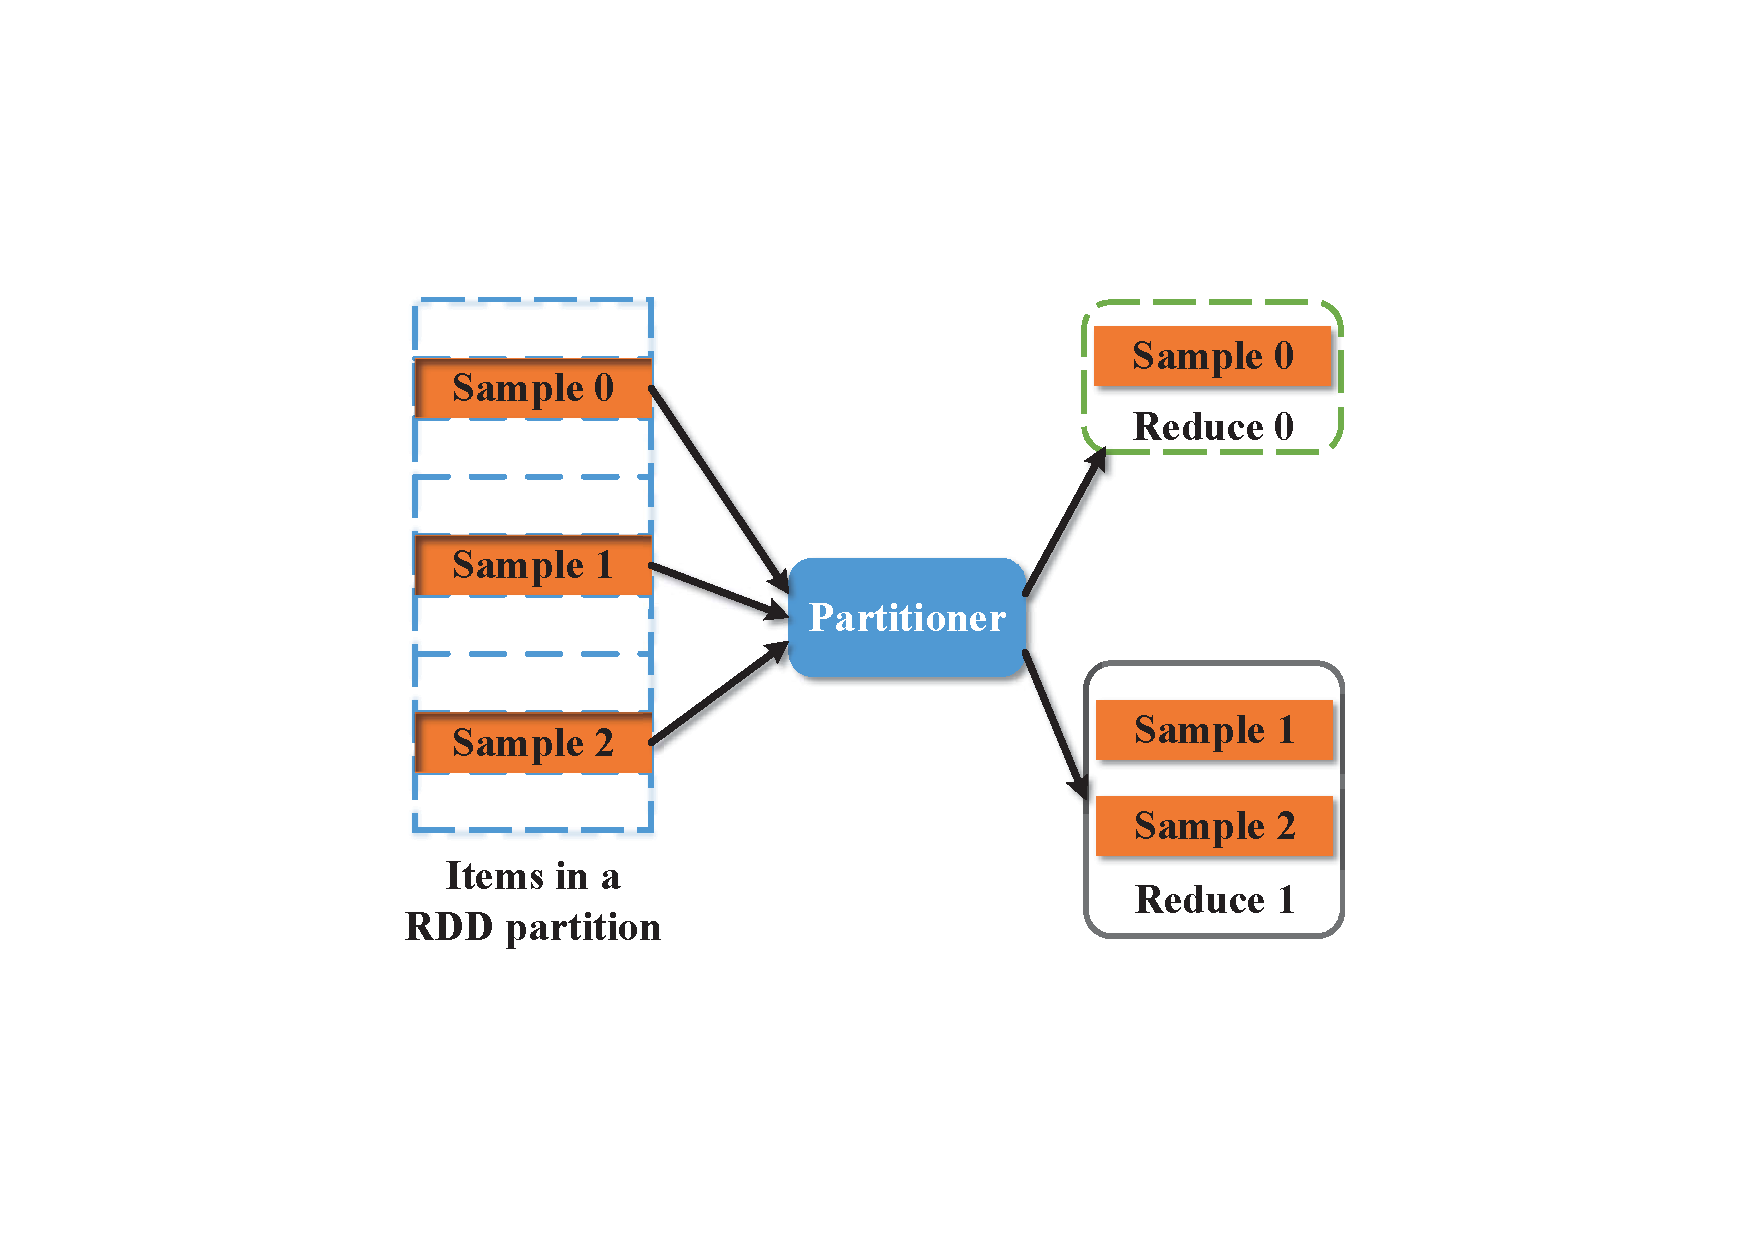
\includegraphics[width=0.6\textwidth]{../../PPoPP-2018/fig/sample.pdf}
	\bicaption[fig:sample]{对于一个任务数据分区的采样}{对于一个任务数据分区的采样}{Fig}{Reservoir Sampling of One Data Partition}
\end{figure}

\section{容错机制}

本小结将从两个角度来讨论SCache在容错性上的设计:Spark执行器或者SCache进程的崩溃造成的错误以及节点崩溃造成的节点下线的错误。

对于Spark执行器发生的错误,SCache采用了独立于Spark执行器的内存空间进行shuffle数据的存储和管理,因此即使Spark的执行器因为错误或者调度原因被Spark主节点杀死或者重启,其中所执行的任务需要的shuffle数据仍然不会遗失。

对于SCache进程的容错性,SCache采用了本地磁盘备份的机制来防止因为错误造成的shuffle数据损失。
当进行shuffle数据块预取的同时,无论该数据块是否在内存中有缓存,SCache都会在节点本地通过异步I/O的方式在本地磁盘对该数据块进行备份。
这些备份会在shuffle数据块被任务使用之后释放。
同时,SCache的工作节点会定期向主节点发送心跳信息,一旦主节点没有收到其中一个工作节点的心跳,就可以通过远程脚本控制其在本地重启。
当工作节点重启之后,主节点会向其发送当前shuffle的调度状态,工作节点则会根据本地磁盘的shuffle数据块备份状况和当前的shuffle状态来判断是否有未完成的shuffle数据块预取以及缓存任务。
而在工作节点进程失效的过程中,Spark的执行器如果有相应的reduce任务执行需要数据,则会被其中的守护进程阻塞住,直到本地工作进程完成重启。
对于SCache主节点的容错性,由于主节点的进程只服务与一个Spark的Driver程序,并且不需要调度对于跨工作的shuffle数据依赖,因此主节点采用了简单的本地磁盘备份日志的方式来备份当前对于相关shuffle的元数据记录和调度记录等信息。

为了降低系统复杂度,SCache在设计的过程中并未引入应对节点崩溃下线的容错机制。
省略这部分机制的原因主要有一下几点:
\begin{itemize}
    \item 备份机制的开销过大,与优化shuffle过程的性能目标相对立。在设计系统的过程中我们并未加入比如经典的GFS\cite{gfs}中提出的三备份机制。
    采用此类容错机制虽然能提升系统的鲁棒性,但是同时也会增加系统在执行shuffle预取与缓存过程中的开销。
    比如如果采用三备份机制,那么在shuffle数据预取阶段以及本地shuffle存储的开销都会随着备份数目的增加而倍增。
    虽然在章节\ref{subsec:size}中我们发现shuffle数据体积对较小,但是备份机制带来的额外开销无疑会给数据中心网络的性能甚至内存和硬盘的性能带来一定挑战,这也与我们的优化目标相违背。
    \item 需要备份的数据没有复用价值。对于每一个shuffle依赖中的数据,只会在DAG计算过程中被使用一次,之后便会被释放。因此对于这些数据的备份就不像一些复用性较强的存储系统甚至Spark本身的RDD来的重要。
    \item SCache与计算框架的共生性。为了提高效率,SCache采用了与DAG计算框架一一对应的共生设计,即每个计算节点既有DAG计算框架的执行器,又有SCache的工作进程。
    这种共生的模式也意味着当该节点失效时,SCache的工作进程和DAG的计算执行器会同时失效。而DAG计算框架本身又有不同的容错机制来保证任务执行。
    而此时对节点进行备份机制的设计可能不但不利于计算的快速恢复,反而会因为不同的容错策略导致SCache针对节点的容错机制变成无效操作。
    比如在Spark中,当发生数据分区因为错误而遗失是,会采取对失效的RDD分区进行并行恢复的措施。
    在此过程中原来属于一个数据分区的数据会进行再分区,从而加快恢复速度。
    那么此时针对SCache单节点的容错机制即使恢复了丢失的shuffle数据,该份数据在计算中也没有使用价值。
\end{itemize}

虽然在设计中省略了对节点下线的容错性,但是为了保证DAG计算过程在发生错误时仍然能够正确执行,SCache在此处采用了借助DAG计算框架容错性的恢复模式。
比如在上文提到的Spark恢复模式中,该失效的RDD分区会进行一个重新分区的并行计算,而在次过程中,SCache对于shuffle的优化将对这部分逻辑进行重新提交和分配。
通过借助DAG计算框架本身的容错性,SCache能保证在节点下线的恢复过程中不破坏任务的正确性,同时提供对恢复中的shuffle优化。

\section{普适性分析}
\label{sec:impl}

为了验证本研究方案的普适性,本章将详细展示在工程方面改造Spark的开销。
同时也将展示在Hadoop MapReduce上的可行性分析。
通过以上两个方面的分析和探索,最终可以证明SCache提供的优化方案可以在不需要大量改造成本的情况下即可适配目前主流的分布式DAG框架。

\subsection{Spark的实现分析}
本次实现中,我们利用Spark这个被广泛应用的分布式DAG计算平台来对SCache的优化进行适配。
在Spark上的修改主要集中在以下几个方面。

首先,我们通过netty\cite{netty}的RPC库在Spark内部实现了一个守护进程 --- \verb|ScacheDaemon|。
在\verb|ScacheDaemon|中,我们实现了表格\ref{tab:apis}中的相应接口,具体代码片段如代码\ref{code:daemon}所示。
其中变量\verb|daemon|是SCache在本地的工作进程,可以通过读取配置文件来获取具体端口,来建立连接,\verb|daemon|本身是一个netty的RPC参考(Reference)实例。
实现中的所有接口都会通过\verb|daemon|这个RPC的参考实例与本地的工作进程和SCache主节点进行数据交互。

\begin{lstlisting}[style={myScalastyle}, caption={ScacheDaemon代码片段}, label={code:daemon}]
    private[spark] class ScacheDaemon (conf: SparkConf) extends Logging {

        val scacheHome = conf.get("spark.scache.home", "~/SCache")
        val platform = "spark"  
        val daemon = new Daemon(scacheHome, platform)   
        val reduceStatus = new ConcurrentHashMap[(Int, Int), mutable.HashMap[Int, Array[String]]]() 
        private var runningJId: Int = -1    
        def setRunningJId(jid: Int): Unit = {
          //Set current runing job id
        }   
        def getRunningJId: Int = runningJId 
        def putBlock (blockId: BlockId, data: Array[Byte], rawLen: Int, compressedLen: Int): Boolean = {
          // Called by Spark Executor
          // The block data is transfered from JVM space of Spark Executor
        }   
        def getBlock(blockId: BlockId): Option[Array[Byte]] = {
          // Called by Spark Executor
          // The block data is fetched from memory of SCache to Spark Executor
        }   
        def registerShuffles(jobId: Int, shuffleIds: Array[Int], maps: Array[Int], reduces: Array[Int], partitioner: Array[String]): Unit = {
          // Called by Spark DAG Scheduler
          // Register shuffle to SCache
        }   
        def getShuffleStatus(jobId: Int, shuffleId: Int): mutable.HashMap[Int, Array[String]] = {
          // Called by Spark Task Scheduler
          // Get pre-scheduled reduce tasks
        }   
    }
\end{lstlisting}

其次,我们修改了Spark的\verb|DAGScheduler|来实现对DAG信息的获取。
具体可以参考如代码\ref{code:dagScheduler}。
在Spark的Driver节点上也存在相应的\verb|Daemon|进程。
当Spark的\verb|DAGScheduler|在从最终的RDD递归向前建立DAG的过程中(\verb|getParentStages|函数),如果发现RDD之前的依赖关系是shuffle依赖,则通过\verb|env.scacheDaemon|
获取本地已经初始化好的守护进程实例,并通过\verb|registerShuffles|接口向SCache提交该shuffle依赖的元数据。

\begin{lstlisting}[style={myScalastyle}, caption={DAGScheduler代码片段}, label={code:dagScheduler}]
    private[spark] class DAGScheduler(...) extends Logging {
            // Skip
            /**
            * Get or create the list of parent stages for a given RDD.  The new Stages will be created with
            * the provided firstJobId.
            */
           private def getParentStages(rdd: RDD[_], firstJobId: Int): List[Stage] = {
             val parents = new HashSet[Stage]
             val visited = new HashSet[RDD[_]]
             val waitingForVisit = new Stack[RDD[_]]
             def visit(r: RDD[_]) {
               if (!visited(r)) {
                 visited += r
                 val shuffles = new ArrayBuffer[ShuffleDependency[_, _, _]]
                 for (dep <- r.dependencies) {
                   dep match {
                     case shufDep: ShuffleDependency[_, _, _] =>
                       parents += getShuffleMapStage(shufDep, firstJobId)
                       shuffles.append(shufDep)
                     case _ =>
                       waitingForVisit.push(dep.rdd)
                   }
                 }
                 if (!shuffles.isEmpty && sc.getConf.getBoolean("spark.scache.enable", false)) {
                   env.scacheDaemon.registerShuffles(firstJobId, shuffles.toArray, rdd.partitions.length, rdd.partitioner.get.toString)
                 }
               }
             }
             waitingForVisit.push(rdd)
             while (waitingForVisit.nonEmpty) {
               visit(waitingForVisit.pop())
             }
             parents.toList
           }
    }
\end{lstlisting}

同时,为了使Spark的执行器在执行map任务时能够将数据发送给SCache,我们实现了一个\verb|ScacheBlockObjectWriter|用来完成map任务的shuffle数据内存拷贝。
\verb|ScacheBlockObjectWriter|实现了对Spark原来的\verb|DiskBlockObjectWriter|的继承,并且重载了其中的方法。
代码\ref{code:writer}展示了\verb|ScacheBlockObjectWriter|在继承过程中对比较重要的几个方法实现了重载。
在这里去掉了原先的磁盘写操作,取代的是对内存缓存空间的数据写入以及内存拷贝,从而优化了map计算任务的磁盘阻塞。

\begin{lstlisting}[style={myScalastyle}, caption={ScacheBlockObjectWriter代码片段}, label={code:writer}]
    class ScacheBlockObjectWriter (...)extends DiskBlockObjectWriter(...) with Logging{
      override def open(): DiskBlockObjectWriter = {
        // Open a byte stream buffer
      }
      override def close(): Unit = {
        // Do memory copy and free memory
      }
      override def write(key: Any, value: Any): Unit = {
        // Write data to byte stream buffer
      }
    }
\end{lstlisting}

而在reduce阶段,我们修改了\verb|ShuffleBlockFetcherIterator|中获取shuffle数据的方法,即调用\verb|ScacheBlockTransferService|中的相应接口来从SCache获取shuffle的数据块。
虽然此处的数据访问通过内存拷贝来完成,但是为了进一步提高性能,以及预防在网络极端拥塞的情况下,最后一轮的几个map任务的输出shuffle数据仍然没有传输完成,在向SCache获取shuffle数据块的时候,
采用了多线程异步非阻塞的方式。
这种实现方式能在第一时间能将已经缓存的shuffle数据块返回给Spark的reduce任务进行计算,因而能将获取shuffle数据时产生对计算的阻塞的可能性降到最低。
代码片段如代码\ref{code:reader}所示。

\begin{lstlisting}[style={myScalastyle}, caption={ScacheBlockTransferService代码片段}, label={code:reader}]
  class ScacheBlockTransferService(daemon: ScacheDaemon) extends Logging{
    def fetchBlocks(
        host: String,
        port: Int,
        execId: String,
        blockIds: Array[String],
        listener: BlockFetchingListener): Unit = {
      // Fetch block from SCache
      // It is a multi-thread asynchronous method that can fetch multiple blocks simultaneously
    }
  }
\end{lstlisting}

在reduce任务预调度方面,Spark的\verb|DAGScheduler.scala|类使其在生成reduce任务时先通过调用RDD的\verb|getPreferedLocs|方法来查询改RDD每个分区对节点的偏好。
而我们通过修改\verb|ShuffleRDD.scala|的\verb|getPreferedLocs|方法,将SCache预调度的结果通过接口\ref{tab:apis}中\verb|getShuffleStatus|返回给RDD。
具体过程可以参考代码\ref{code:preschedule}
获取预调度结果之后,Spark的\verb|TaskSchedulerImpl.scala|就会在调度reduce任务时将其分配到已经完成shuffle数据预取的节点上,从而获得SCache的优化。

\begin{lstlisting}[style={myScalastyle}, caption={Reduce预调度代码片段}, label={code:preschedule}]
    class ShuffledRDD[...](...){
        //Skip
        override protected def getPreferredLocations(partition: Partition): Seq[String] = {
            if (SparkEnv.get.conf.getBoolean("spark.scache.enable", false)) {
              val dep = dependencies.head.asInstanceOf[ShuffleDependency[K, V, C]]
              // Ask SCache to get preferred location
              val locs = SparkEnv.get.scacheDaemon.getShuffleStatusForPartition(dep.shuffleId, partition.index)
              locs.toSeq
            } else {
              val tracker = SparkEnv.get.mapOutputTracker.asInstanceOf[MapOutputTrackerMaster]
              val dep = dependencies.head.asInstanceOf[ShuffleDependency[K, V, C]]
              tracker.getPreferredLocationsForShuffle(dep, partition.index)
            }
        }
    }
\end{lstlisting}

在插入采样程序部分,我们利用了Spark中\verb|RangePartitioner|在决定分区边界时对RDD进行计算的过程,在其中插入了采样过程。
为了提高效率,对RDD数据的采样以及分区的计算是在Spark的Driver内部进行。
计算完成之后再将数据发送给SCache,具体逻辑如代码\ref{code:sample}所示。
其中返回的\verb|distribution|将会作为采样的分布通过接口\ref{tab:apis}中的\verb|sampling|发送给SCache。

\begin{lstlisting}[style={myScalastyle}, caption={水塘采样代码片段}, label={code:sample}]
    def determineBounds[K : Ordering : ClassTag](
        candidates: ArrayBuffer[(K, Float, Int)],
        partitions: Int,
        depPartitionNum: Int): (Array[K], Array[Array[Int]]) = {
      // Skip
      val ordered = candidates.sortBy(_._1)
      val distribution = Array.fill[Int](depPartitionNum)(0)
        .map(x => new Array[Float](partitions))
      var i = 0
      var j = 0
      var previousBound = Option.empty[K]
      while ((i < numCandidates) && (j < partitions - 1)) {
        val (key, weight, index) = ordered(i)
        cumWeight += weight
        distribution(index)(j) += weight
        if (cumWeight >= target) {
          // Skip duplicate values.
          if (previousBound.isEmpty || ordering.gt(key, previousBound.get)) {
            bounds += key
            target += step
            j += 1
            previousBound = Some(key)
          }
        }
        i += 1
      }
      while (i < numCandidates) {
        // calculate the distribution of last partition
        val (key, weight, index) = ordered(i)
        distribution(index)(j) += weight
        i += 1
      }
      (bounds.toArray, distribution)
    }
\end{lstlisting}

以上四个部分是在Spark适配过程中做出的主要改动,其代码量大约在1000行左右,相较于Spark本身几十万行的代码量,可以说这个改动是非常的小。

\subsection{Hadoop MapReduce的可行性分析}

受限于时间,本研究并没有对Hadoop MapReduce进行SCache的适配改造。
但是为了验证SCache对shuffle的优化的普适性,本研究仍对Hadoop MapReduce的适配可行性进行了分析研究。

首先,我们对Hadoop MapReduce的计算过程中存在的shuffle特点进行分析。
虽然在表达DAG的过程中Hadoop MapReduce与Spark存在较大差异,但是在每个map和reduce的计算阶段之间都会存在一个shuffle的过程却十分接近。
在执行map任务时,Hadoop MapReduce中的\verb|MapTask.java|类
会将map任务计算产生的shuffle结果通过\verb|MapOutputClollector.java|接口写入到本地磁盘进行保存。
当reduce任务数目不为0时,即该map阶段不是分布式应用的最后一次计算阶段时,map任务会调用\verb|NewOutputCollector.java|来写入该阶段的输出键值对。
在具体执行过程中,其通过实例化一个\verb|collector|来进行写操作,而该\verb|collector|就是一个\verb|MapOutputClollector.java|的具体实例。
具体代码参考代码片段\ref{code:hadoopmap}

在reduce阶段,每个reduce任务由类\verb|ReduceTask.java|来执行。
具体来说,每个reduce任务会通过\verb|ShuffleConsumerPlugin|的接口来实现第一阶段的远程shuffle数据拷贝过程。
在目前的MapReduce中,该接口由类\verb|Shuffle<K, V>|实现了一个多线程的异步远程shuffle数据读取。
具体可以参考代码片段\ref{code:hadoopreduce}。

\begin{lstlisting}[language={Java}, caption={Hadoop MapReduce中Map阶段的shuffle写代码片段}, label={code:hadoopmap}]
    private <...>
    void runNewMapper(...) throws IOException, ClassNotFoundException,
                             InterruptedException {
        // Skip
        // get an output object
        if (job.getNumReduceTasks() == 0) {
          output = 
            new NewDirectOutputCollector(taskContext, job, umbilical, reporter);
        } else {
          output = new NewOutputCollector(taskContext, job, umbilical, reporter);
        }
        // Skip    
        try {
          long startTime = System.currentTimeMillis();
          input.initialize(split, mapperContext);
          mapper.run(mapperContext);
          mapPhase.complete();
          setPhase(TaskStatus.Phase.SORT);
          statusUpdate(umbilical);
          input.close();
          input = null;
          output.close(mapperContext);
          output = null;
        } finally {
          closeQuietly(input);
          closeQuietly(output, mapperContext);
        }
    }

    NewOutputCollector(...) throws IOException, ClassNotFoundException {
        @Override
        public void write(K key, V value) throws IOException, InterruptedException {
          collector.collect(key, value,
                            partitioner.getPartition(key, value, partitions));
        }
        @Override
        public void close(TaskAttemptContext context
                          ) throws IOException,InterruptedException {
          try {
            collector.flush();
          } catch (ClassNotFoundException cnf) {
            throw new IOException("can't find class ", cnf);
          }
          collector.close();
        }
    }
\end{lstlisting}

\begin{lstlisting}[language={Java}, caption={Hadoop MapReduce中Reduce阶段的shuffle读代码片段}, label={code:hadoopreduce}]
    public class ReduceTask extends Task {
        public void run(...) throws IOException, InterruptedException, ClassNotFoundException {
          // Skip
          ShuffleConsumerPlugin.Context shuffleContext = new ShuffleConsumerPlugin.Context(...);
          shuffleConsumerPlugin.init(shuffleContext);
          // fetch the remote shuffle blocks simultaneously
          rIter = shuffleConsumerPlugin.run();
        }
    }

    public class Shuffle<K, V> implements ShuffleConsumerPlugin<K, V>, ExceptionReporter {
        // Skip
        @Override
        public RawKeyValueIterator run() throws IOException, InterruptedException {
          //Skip
          if (isLocal) {
            fetchers[0] = new LocalFetcher<K, V>(jobConf, reduceId, scheduler,
            merger, reporter, metrics, this, reduceTask.getShuffleSecret(),
            localMapFiles);
            fetchers[0].start();
          } else {
            for (int i=0; i < numFetchers; ++i) {
              fetchers[i] = new Fetcher<K,V>(...);
              fetchers[i].start();
            }
          }
        }
    }
\end{lstlisting}

而对于任务的调度,在Hadoop MapReduce中,主要由一系列状态机的转移和Yarn\cite{yarn}的资源调度机制协同完成。
具体来讲,在一个MapReduce任务被提交之后,经过一系列的状态转移,最终会由\verb|JobImpl|类来完成map和reduce阶段的具体任务生成以及提交。
而由于MapReduce的计算DAG相较于Spark十分简单,即在一个任务只有Map和Reduce两个过程,所以对于shuffle的相关元数据便可以在此处获得。
具体关于shuffle两端map和reduce任务的生成,可以参考代码\ref{code:hadoopshuffle}。

\begin{lstlisting}[language={Java}, caption={Hadoop MapReduce中shuffle元数据生成代码片段}, label={code:hadoopshuffle}]
    public class JobImpl implements org.apache.hadoop.mapreduce.v2.app.job.Job, EventHandler<JobEvent> {
        // Skip
        @Override
        public JobStateInternal transition(JobImpl job, JobEvent event) {
          // Skip
          createMapTasks(job, inputLength, taskSplitMetaInfo);
          createReduceTasks(job);
        }
    }
\end{lstlisting}

对于reduce阶段的任务预调度,在MapReduce中都是通过\verb|RMContainerAllocator.java|的类来实现的。
当其收到对reduce任务的调度的请求时,\verb|RMContainerAllocator.java|会根据从Yarn的ResourceManager那里获取的可用容器数(Container)进行分配。
具体可以参考代码片段\ref{code:hadoopschedule}

\begin{lstlisting}[language={Java}, caption={Hadoop MapReduce中reduce任务调度代码片段}, label={code:hadoopschedule}]
    public class RMContainerAllocator extends RMContainerRequestor implements ContainerAllocator {
        private ContainerRequest assignToReduce(Container allocated) {
          ContainerRequest assigned = null;
          //try to assign to reduces if present
          if (assigned == null && reduces.size() > 0 && canAssignReduces()) {
            TaskAttemptId tId = reduces.keySet().iterator().next();
            assigned = reduces.remove(tId);
            LOG.info("Assigned to reduce");
          }
          return assigned;
        }
    }
\end{lstlisting}

综上所述,我们给出了一下对Hadoop MapReduce的SCache适配的改造方案。
\begin{enumerate}
    \item Shuffle元数据获取:在\verb|JobImpl|类中发生任务提交而产生的状态转换函数执行过程中,可以获取shuffle两端对应的map任务个数,reduce任务个数等信息。
    此时,便可以将这些数据通过接口\ref{tab:apis}中的\verb|registerShuffles|进行提交。
    \item Map任务shuffle数据的解耦:可以通过重新实现一个对接口\verb|MapOutputClollector|的实现类来获取shuffle数据,并且通过内存拷贝传递给SCache。
    \item Reduce任务shuffle数据的解耦:可以通过重新实现一个接口\verb|ShuffleConsumerPlugin|的实现类来从SCache的内存缓存获取shuffle的数据。
    \item Reduce任务的预调度:需要将SCache的预调度结果通过接口在\verb|RMContainerAllocator.java|调度任务前对预调度结果进行获取,然后在其调用\verb|assignToReduce|函数时遵循预调度的结果即可。
    \item 采样任务的实现:在\verb|JobImpl|类中生成具体任务的时候,可以通过配置信息来获取分区函数的信息。
    如果发现是一个非哈希的分区函数,则在创建map任务的同时创建每个任务对应的采样任务对其进行数据采样。
\end{enumerate}

以上两个小节通过对目前最流行的Spark和Hadoop MapReduce这两个典型的分布式DAG计算框架应用SCache优化的可行性做出了具体的分析。
通过展现Spark上的具体实现技术,可以看到应用SCache的优化对于原有框架本身并不需要做出巨大的修改。
同时,通过对Hadoop MapReduce的任务执行框架任务调度流程,shuffle过程的分析,我们发现对于SCache提供的优化策略在Hadoop MapReduce上也能非常方便的适配。
因此我们认为SCache提供的优化方案对于目前主流的分布式DAG计算框架具有较好的普适性。
能够通过对现有框架较少的改动而实现适配与shuffle的优化。